\chapter{Methodology} \label{Chap3}
One of the main challenges in transpilation is mapping logical qubits to physical qubits, especially since physical qubits often have limited connectivity. The qubit-mapping problem is classified as NP-hard \cite{botea_complexity_2021}, meaning that while optimal solutions may be achievable for small quantum circuits, the problem becomes increasingly difficult for larger circuits. Because most quantum hardware only allows two-qubit gates to operate between physically adjacent qubits, two important strategies are required: determining the initial placement of qubits and inserting swap gates when a gate execution violates these connectivity constraints \cite{cowtan_qubit_2019}.

For the overview of the algorithms, the initial step in addressing the qubit-mapping problem involves utilizing the physical qubit connectivity and gate priorities to generate an initial qubit mapping that is more efficient than a simple one-to-one layout. The subsequent step introduces a dynamic lookahead window to insert swap gates more efficiently taking into account gates that give positive effect to the swap candidate. This proposed algorithms successfully address the coupling limitations of quantum devices and reduce the overhead of inserting swap gates, leading to better performance on networked quantum hardware.

Table \ref{tab:definition-notation} provides the definitions for the notations used in the analysis:
\begin{table}[htb]
\centering
\caption{Definition of Notations}
\label{tab:definition-notation}
\begin{tabular}{|l|l|} 
\hline
\textbf{Notation} & \textbf{Definition}                                            \\ 
\hline
$n$               & number of logical qubits                                       \\ 
\hline
$q_{1,2,...,n}$     & logical qubits $q_L$ in quantum circuit                        \\ 
\hline
$N$               & number of physical qubits                                      \\ 
\hline
$Q_{1,2,...,N}$     & physical qubits $Q_P$ on quantum device                        \\ 
\hline
$C_{1,2,...,N}$     & classical register for quantum device                          \\ 
\hline
$g_i$             & number of gates in the circuit                                 \\ 
\hline
$d$               & depth of the circuit                                           \\ 
\hline
$G(V, E)$         & the coupling graph of the backend                              \\ 
\hline
$D[\ ][\ ]$       & the distance matrix of the physical qubits between $Q_i, Q_j$  \\ 
\hline
$\pi()$           & a mapping from $q_{1,2,...,n}$ to $Q_{1,2,...,N}$                  \\ 
\hline
$\pi^-1()$        & a mapping from $Q_{1,2,...,N}$ to $q_{1,2,...,n}$                  \\ 
\hline
$F$               & Front layer of quantum circuit                                 \\
\hline
\end{tabular}
\end{table}

\section{Layout}
% \cite{peham_optimal_2023} FOR LAYOUT RING STRUCTURE DST
\subsection{Distributed Coupling Graph} % done chat
Simulating a distributed quantum computer involves creating a coupling map that represents the connectivity of qubits across different "groups", with each group acting as a separate node or quantum processor within the quantum network. These groups consist of multiple \acrfull{qpu}, with connections both within each group and between different groups. The coupling graph defines the topology of the \acrshort{qpu} within each group, and this is managed using \lstinline{CouplingMap} \cite{ibmquantum_couplingmap} class in Qiskit. In this coupling graph, the last qubit of one group is connected to the first qubit of the next group, forming a larger distributed coupling map. By modifying the internal topology of a node (quantum computer) and the distribution of qubits across different groups, various configurations of the quantum network can be explored, as illustrated in Appendix \ref{app:coupling-graph-by-group}. \\
The following functions are used to define the topology within each group:
\begin{itemize}[noitemsep,nolistsep]
    \item \lstinline{from_line}: creates a coupling map of $n$ qubits connected in a line.
    \item \lstinline{from_grid}: creates a coupling map of qubits arranged in a grid with a specified number of rows and columns.
    \item \lstinline{from_ring}: creates a coupling map of $n$ qubits connected in a ring.
    \item \lstinline{from_full}: creates a fully connected coupling map on $n$ qubits.
    \item \lstinline{from_t_horizontal}: creates a coupling map of five qubits arranged in a T-shape, connected at the longer end.
    \item \lstinline{from_t_vertical}: creates a coupling map of five qubits arranged in a T-shape, connected at the shorter end.
\end{itemize}

\subsection{Interaction Mapping} % done chat
In this section, an algorithm called \mycode{InteractionLayoutMapping} will be discussed to determine the most appropriate mapping from logical qubits to physical qubits. During the initialization step, the connectivity of the physical qubits on the backend is determined, and the priority of two-qubit gates is assigned based on their order of appearance in the quantum circuit, with gates appearing earlier (on the left side) being given higher priority \cite{liu_qm-dla_2024}. Additionally, a metric is calculated to measure qubit interactions that quantify how qubits interact with each other within a circuit, particularly on how qubits are connected through multi-qubit gates, such as CNOT gates \cite{bandic_interaction_2023}. This calculation will help to define the order in which quantum gates are prioritized.

\begin{definition} % done chat
    Physical connectivity is the number of neighbours of physical qubits ($Q_P$).
\end{definition}
A physical quantum device is represented by a coupling graph, which is a directed graph (V, E). In this graph, $Q = \{Q_0, Q_1, ..., Q_{N-1}\}$ represents the set of physical qubits as vertices (V), and the edges (E) represent the direct connections between two physical qubits, $Q_i$ and $Q_j$, where a two-qubit gate can be applied. When a physical qubit has higher connectivity, the logical qubit mapped to it has a greater chance of connecting to other logical qubits without needing additional swap gates. Conversely, if a physical qubit has low connectivity, more qubit movements will be needed to satisfy the coupling constraints before a logical gate can be operated. These additional movements increase the need for swap gate insertions, leading to a larger circuit size and depth, which may negatively impact gate fidelity and runtime. For example, Qiskit \lstinline{FakeLondonV2} \cite{ibmquantum_fakelondonv2} (Figure \ref{fig:fake-london})  is a simulated 5-qubit backend with a coupling graph that illustrates the physical connectivity on each qubit.
\begin{figure}[h]
    \centering
    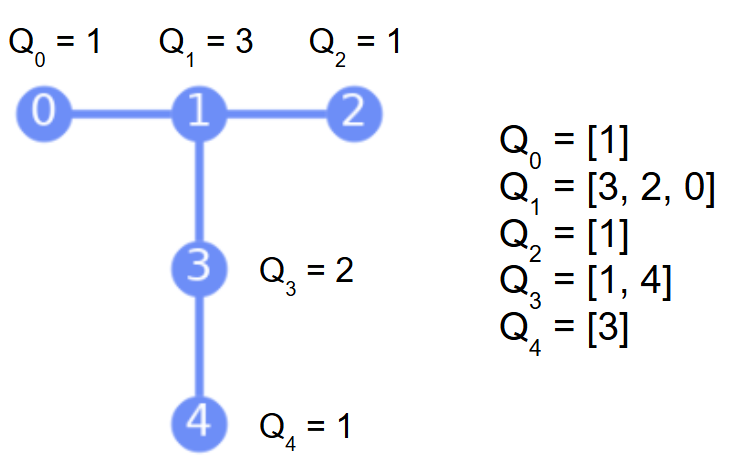
\includegraphics[width=0.4\linewidth]{image/fake_london.png}
    \caption{\lstinline{FakeLondonV2} coupling map and its physical connectivity list containing the number of neighbours of each physical qubit $Q_P$.}
    \label{fig:fake-london}
\end{figure}

\begin{definition} % done chat
    Logical priority calculates the number of two-qubit gates acting on each logical qubit in a quantum circuit.
\end{definition}
If two logical qubits have the same priority value, the one with the earlier index is given precedence. The logical neighbours list identifies other logical qubits that interact with a specific logical qubit $q_i$ in the circuit. Figure \ref{fig:logical-priority} lists the number two-qubit gates operating on the wire of the quantum circuit.
\begin{figure}[h]
    \centering
    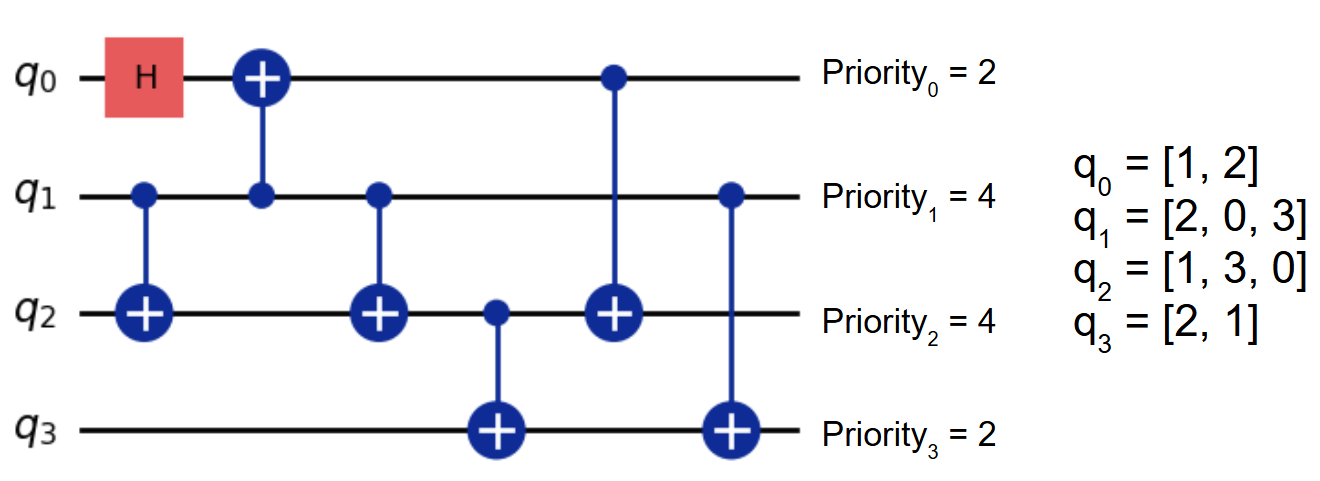
\includegraphics[width=0.7\linewidth]{image/logical_priority.png}
    \caption{Logical priority of a quantum circuit and its logical neighbours list containing the indices of qubits that interact with the logical qubit $q_i$.}
    \label{fig:logical-priority}
\end{figure}

\begin{definition} % done chat
    Gate weight reflects the importance of each gate $g_i$ in a quantum circuit, based on when it occurs in the sequence of operations.
\end{definition}
In a quantum circuit, consider a set of logical qubits $q_L = \{q_0, q_1, ..., q_{n-1}\}$ and an ordered sequence of gates $g = \{g_0, g_1, ..., g_{m-1}\}$. It is important to note that the ordering of gates introduces some arbitrariness, as certain gates can be implemented in parallel. For example, the last two gates in Figure \ref{fig:gate-weight}, CNOT $(q_0, q_2)$ and CNOT $(q_1, q_3)$, could be executed simulatenously, making the weights of $g_6$ and $g_7$ interchangeable. \\
Each quantum gate $g_i$ is assigned a weight $w_i$, which is calculated as:
\begin{equation}
    w_i = m - i
\end{equation}
where $m$ is the total number of gates in the quantum circuit, and $i$ is the gate's position in the sequence. A higher weight suggests that the gate occurs earlier in the sequence, potentially having a greater influence on the subsequent operations and the final state of the quantum system. Figure \ref{fig:gate-weight} shows the gate weights in descending order, with earlier gates assigned higher values.
\begin{figure}[h]
    \centering
    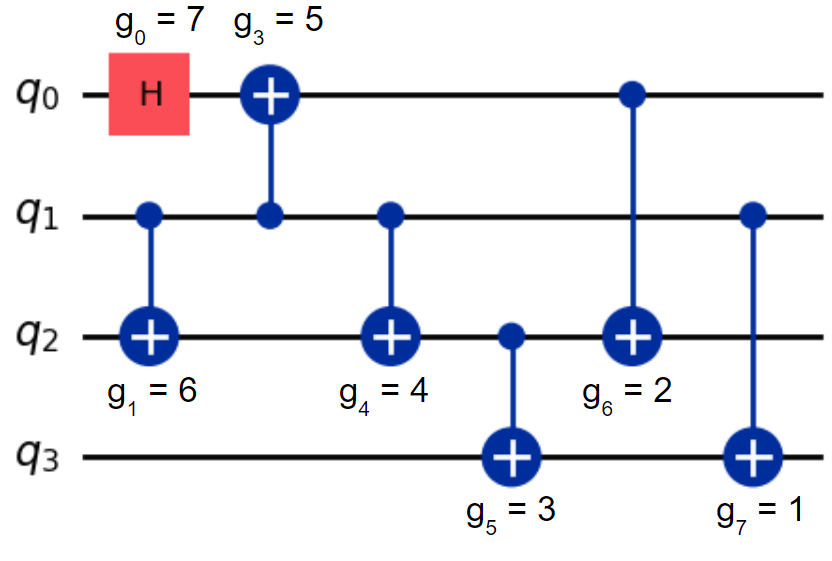
\includegraphics[width=0.4\linewidth]{image/gate_weight.png}
    \caption{Gate weight of a quantum circuit, with front gates assigned higher weights}
    \label{fig:gate-weight}
\end{figure}
\begin{definition}
    \acrfull{qpi} refers to the measure of interaction logical qubit pair (q\textsubscript{i}, q\textsubscript{j}) when they are involved in a multi-qubit quantum gate, such as controlled-NOT (CNOT) gate or any other two-qubit gate.
\end{definition}
\acrshort{qpi} is determined by summing all gate weights that involve the qubit pair and is represented as a 2D matrix, as in Table \ref{tab:qpi-matrix}:
\begin{equation}
    \text{QPI}(q_i, q_j) = \sum_{k \in \mathcal{G}(q_i, q_j)} w_k
\end{equation}
where $\mathcal{G}(q_i, q_j)$ represents the set of indices $k$ corresponding to gates that involve both qubits $q_i$ and $q_j$, and $w_k$ is the weight of gate $g_k$. \\
\begin{table}[h]
    \centering
    \begin{tabular}{|c|c|c|c|c|c|}
        \hline
        $(q_i, q_j)$ & (0, 1) & (0, 2) & (1, 2) & (1, 3) & (2, 3) \\
        \hline
        QPI & 5 & 2 & 10 & 1 & 3 \\
        \hline
    \end{tabular}
    \caption{\acrshort{qpi} value of gates on logical qubits $(q_i, q_j)$ from quantum circuit on Figure \ref{fig:gate-weight}.}
    \label{tab:qpi-matrix}
\end{table}
\begin{definition}
    \acrfull{qbn} refers to the sum of weights of the qubit pairs interactions (\acrshort{qpi} values) that involve the logical qubit being considered and its neighbouring physical qubits.
\end{definition}
A higher \acrshort{qbn} value indicates that the qubit is more connected or plays a more significant role within the quantum circuit. The \acrshort{qbn} value is defined as:
\begin{equation}
    \text{QBN}(q_i) = \sum_{j} \text{QPI}(q_i, Q_{P,j})
\end{equation}
where $q_i$ is the logical qubit under consideration, $Q_{P,j}$ denotes each physical qubit that is adjacent to or interacts with $q_i$, and $\text{QPI}(q_i, Q_{P,j})$ represents the interaction strength (weight) between $q_i$ and the $j$-th adjacent physical qubit.

\subsection{Interaction Mapping Algorithm}
Algorithm \ref{alg:interaction-layout-mapping} \mycode{InteractionLayoutMapping} outlines the steps for creating an initial qubit mapping, where the inputs are the device's coupling map and the circuit's \acrfull{dag}, and the output is a layout that maps logical qubits $(q_L)$ to physical qubits $(Q_P)$. The algorithm starts by calculating physical connectivity from the coupling map and determining the logical qubits' priorities, which are sorted in descending order. The logical qubit with the highest priority is then mapped to the physical qubit with the most connections. For subsequent placements, the algorithm checks if the assigned physical qubits have adjacent neighbours. If they do, it evaluates \acrfull{qpi} between the logical neighbours and their corresponding qubits, selecting the highest QPI candidate for mapping. If no adjacent neighbours meet this criterion, the algorithm assigns the next highest physically connected qubits to the logical qubits. This process generates all possible mappings for the quantum circuit, which are then ranked based on their total QPI index, and the final output is one initial mapping with the highest QPI rank. If multiple mappings have the same top QPI rank, the final output may be different with each run.

\begin{algorithm}[htb]
\caption{Interaction Layout Mapping}\label{alg:interaction-layout-mapping}
\hspace*{\algorithmicindent} \textbf{Input} Coupling Graph G(V, E), Circuit DAG \\
\begin{algorithmic}[1]
\State physical connectivity $\gets E$ on $Q_P$
\State logical priority $\gets g$ on $q_L$
\If{coupling graph is mostly fully connected}
\State \Return one-to-one index mapping
\EndIf
\State maps = [\ ]
\While{logical priority is not empty}
    \For{maps}
        \State $q_i \gets$ max (logical priority)
        \State temp physical connectivity $\gets$ neighbours of assigned $Q_P$
        \If{all $q_i$ neighbours already assigned}
            \State $Q_X \gets$ max(temp physical connectivity)
            \State maps $\gets (q_i, Q_X)$
        \Else
            \State $Q_X$ neighbours[\ ] $\gets$ adjacent assigned $Q_P$
            \State Get all assigned $q_L$ from maps
            \For{available $Q_X$ neighbours}
                \State $q_j \gets \pi^{-1}(\text{available }Q_X)$
                \State QBN candidate $\gets \text{QPI}[q_i][q_j]$
            \EndFor
            \State $Q_X \gets$ max (QBN value)
            \State maps $\gets (q_i, Q_X)$
        \EndIf
    \EndFor
\EndWhile
\end{algorithmic}
\end{algorithm}

\begin{example} % done chat
The initial quantum circuit shown in Figure \ref{fig:circuit-init} is processed through Algorithm \ref{alg:interaction-layout-mapping} \mycode{InteractionLayoutMapping} to obtain a more efficient solution for qubit placement. The backend device used is a simulated five-qubit system, \lstinline{FakeLondonV2}. \\
First, logical qubit $q_1$ is directly assigned to $Q_1$, which has the most connections with three neighbours. The current mapping is $[[\colorbox{backcolour}{(1, 1)}]]$, where the first value in the tuple represents the logical qubit $(q_L)$ and the second value represents the physical qubit $(Q_P)$. Next, logical qubit $q_2$ is to be assigned to the available physical candidates $Q_3$, $Q_2$, and $Q_0$. The \acrshort{qpi}$(q_1, q_2)$ value is 10 for all these candidates, so they are all included in the mapping. The current mapping is $[[(1, 1), \colorbox{backcolour}{(2, 3)}], [(1, 1), (2, 2)], [(1, 1), (2, 0)]]$, and the sum of \acrshort{qbn} is recorded. Figure \ref{fig:circuit-mapping} illustrates the path when physical qubit $Q_3$ is chosen for logical qubit $q_2$. The next logical qubit, $q_0$, has possible physical candidates $Q_0$, $Q_2$, and $Q_4$. Using the mapped logical qubits and their assigned physical qubits, the \acrshort{qpi} values are calculated, and the \acrshort{qbn} values are summed to determine the maximum value. For the neighbour of $Q_1$, the \acrshort{qpi} between $q_0$ and $q_1$ is 5, while for the neighbor of $Q_3$, the \acrshort{qpi} between $q_0$, $q_2$ is 2. The maximum value occurs for both $Q_0$ and $Q_2$. Therefore, the updated mapping for path $[(1, 1), (2, 3)]$ is $[[(1, 1), (2, 3), \colorbox{backcolour}{(0, 2)}], [(1, 1), (2, 3), (0, 0)]]$. With the last mapping of $(q_0, Q_2)$, the last logical qubit is for $q_3$ has available candidates $Q_0$ and $Q_4$. If $q_3$ is assigned to $Q_0$, the \acrshort{qpi} value is 1, while for $Q_4$, the \acrshort{qpi} value is 3. The final assignment is $(q_3, Q_4)$ and \acrshort{qbn} rank is updated accordingly. The algorithm not only generates all possible paths for mapping but also identifies the path with the highest \acrshort{qbn} rank. The chosen layout is $[(1, 1), (2, 3), (0, 0), \colorbox{backcolour}{(3, 4)}]$, as shown in Figure \ref{fig:plot-circuit-layout}, with a total rank of $18.0$. The initial quantum circuit is redrawn as in Figure \ref{fig:circuit-layout-isa}.
\end{example}

\begin{figure}[htbp]
    \centering
        \begin{subfigure}{0.6\linewidth}
        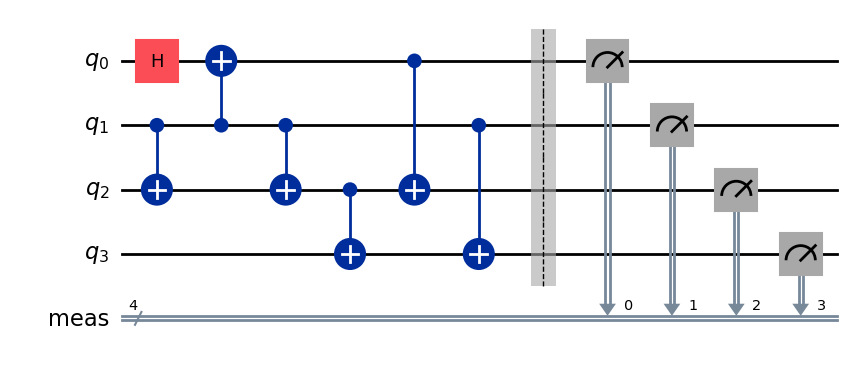
\includegraphics[width=\linewidth]{image/circuit_init.png}
        \caption{Initial quantum circuit}
        \label{fig:circuit-init}
    \end{subfigure}
    \vspace{1em}
    \begin{subfigure}{0.8\linewidth}
        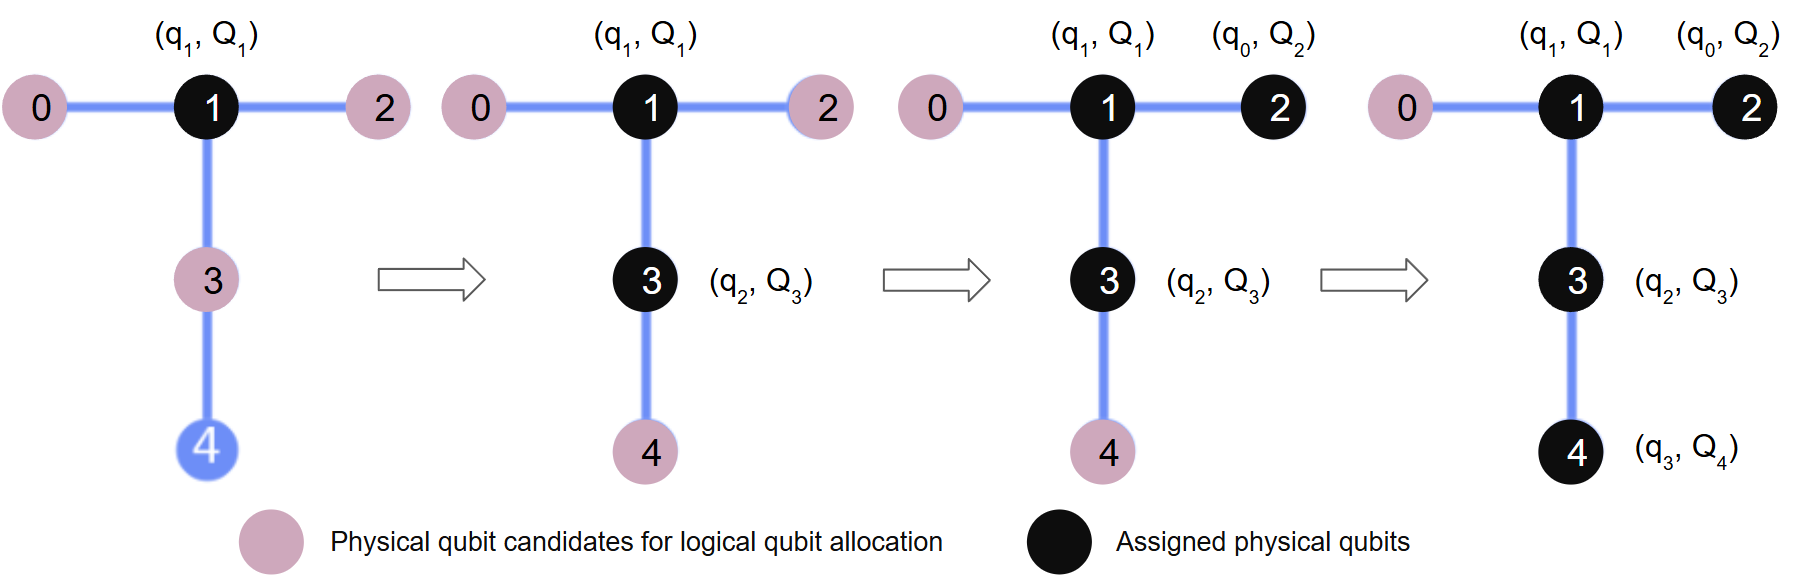
\includegraphics[width=\linewidth]{image/circuit_mapping.png}
        \caption{Steps to assign logical qubit to backend coupling map}
        \label{fig:circuit-mapping}
    \end{subfigure}
    \vspace{1em}
    \begin{subfigure}{0.6\linewidth}
        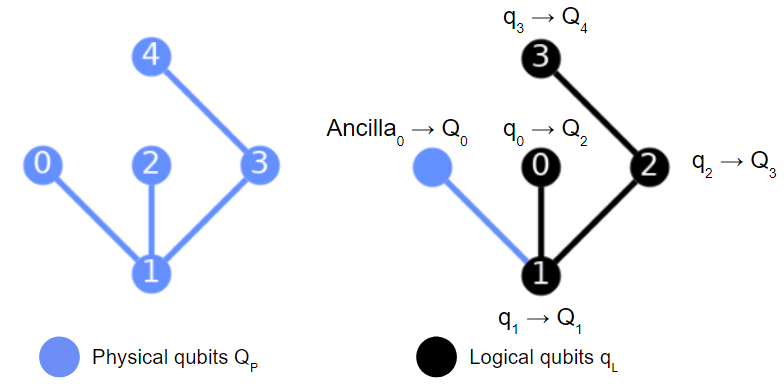
\includegraphics[width=\linewidth]{image/plot_circuit_layout.png}
        \caption{$\pi(q_L, Q_P)$ mapping in the coupling map, where the blue nodes on the left are physical qubits $Q_P$, and the black nodes on the right are logical qubits $q_L$ assigned to the physical qubits.}
        \label{fig:plot-circuit-layout}
    \end{subfigure}
    \vspace{1em}
    \begin{subfigure}{0.6\linewidth}
        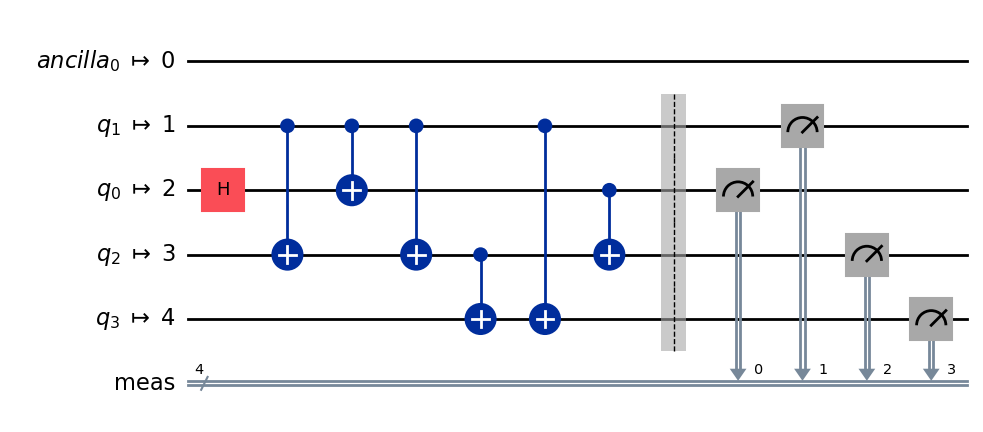
\includegraphics[width=\linewidth]{image/circuit_layout.png}
        \caption{Redraw quantum circuit in embed coupling map}
        \label{fig:circuit-layout-isa}
    \end{subfigure}
    \caption{Interaction layout mapping $(q_L, Q_P)$}
\end{figure}

\subsection{Analysis Pass} % done chat
Qiskit framework provides specific \lstinline{AnalysisPass} \cite{ibmquantum_analysispass} to change the property set of a quantum circuit. The custom analysis pass requires layout mapping as input, builds the mapping to Qiskit \lstinline{Layout} \cite{ibmquantum_layout} class, and implements the abstract run function. The class layout constructs a bijective dictionary, mapping virtual qubits $q_L$ to physical qubits $Q_P$. An AnalysisPass might be used to evaluate the effectiveness of a given qubit layout, guiding the optimization process and ensuring that the final circuit is well-suited for the physical quantum hardware it will run on.

\newpage
\section{Routing}
\subsection{Lookahead Swap}
When addressing the qubit mapping problem, all two-qubit gates must meet the hardware connectivity constraints. Single-qubit gates, which act on individual physical qubits, are not relevant and can be ignored for the mapping problem. In most cases, it is not feasible to find a mapping that satisfies all connectivity constraints for the entire quantum circuit. Therefore, whenever a gate does not meet these constraints, the mapping between logical and physical qubits must be updated using swap gates. However, adding swap gates can greatly affect the order of subsequent logical gates. The main metrics for evaluating these adjustments are the number of additional swap gates needed and the resulting circuit depth.

% from chat
\begin{definition}
    DAGCircuit \cite{ibmquantum_dagcircuit} is a \acrfull{dag} representation of a quantum circuit. This intermediate representation allows the manipulation and optimization of quantum circuits.
\end{definition}
In the \acrshort{dag}, each node corresponds to a quantum gate or a measurement applied to qubits, while the edges indicate the flow of quantum information between operations, connecting the output of one operation to the input of another. The \acrshort{dag} structure can be analysed by counting the number of qubits and assessing the circuit depth, which may help simplify the circuit by merging gates, eliminating redundant operations, and applying other techniques to reduce the circuit's complexity \cite{li_tackling_2019}. Figure \ref{fig:dag-embeded} illustrates the flow of a quantum circuit, where green nodes represent logical qubit inputs, blue nodes represent logical gates $g$, and red nodes represent logical qubit outputs. The edges in the graph depict the quantum information flow from input to output. Additionally, each level in the graph corresponds to the quantum circuit depth, so when multiple nodes appear at the same level, it indicates that the gate operations are applied to disjoint physical qubits.
\begin{figure}[h]
    \centering
    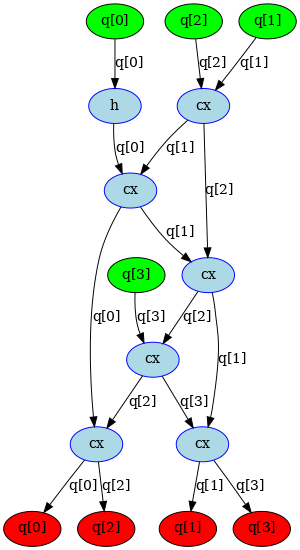
\includegraphics[width=0.3\linewidth]{image/dag_embeded.png}
    \caption{\acrfull{dag} of the previous quantum circuit (Figure \ref{fig:circuit-init}). \acrshort{dag} consists of three nodes: \acrshort{dag} input nodes (green), \acrshort{dag} operation nodes (blue), and \acrshort{dag} output nodes (red). The arrows indicate the quantum information flow.}
    \label{fig:dag-embeded}
\end{figure}

\begin{definition}
    The Gate Front Layer refers to a series of quantum gates that have no pending predecessors on their associated qubits.
\end{definition}
A layer in a quantum circuit consists of gates that operate on non-overlapping qubits, and the total number of layers corresponds to the circuit depth, denoted as \textit{d}. From Qiskit documentation, these layers are generated using a greedy algorithm. The resulting layer includes new \acrshort{dag} operation nodes, \acrshort{dag} input nodes, and \acrshort{dag} output nodes. In the \acrshort{dag} illustrated in Figure \ref{fig:dag-embeded}, the front layer consists of the $CX$ and $H$ gates.

\begin{definition} % done chat
    Nearest neighbour distance refers to the shortest distance between a given qubit and its closest neighbouring qubit in a quantum device. 
\end{definition}
In most quantum hardware, two-qubit gates (like CNOT or CZ gates) can only be directly implemented between qubits that are physically adjacent. If the two qubits involved in the gate are not neighbours, they need to be moved closer together through a series of SWAP operations, which exchange the positions of qubits on the device. \\
In the setup Figure \ref{fig:nearest-neighbour-distance}, the nearest neighbour distance between $Q_0$ and $Q_1$ is 1, the nearest neighbour distance between $Q_1$ and $Q_2$ is 1, and the nearest neighbour distance between $Q_0$ and $Q_2$ is 2, as they are not direct neighbours.
\begin{figure}[htb]
    \centering
    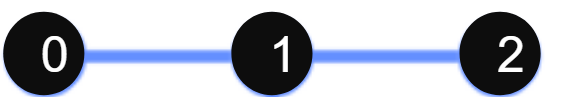
\includegraphics[width=0.25\linewidth]{image/nearest_neighbour_distance.png}
    \caption{Example of nearest neighbour distance setup, where distance $Q_0 - Q_1$ is 1, and distance $Q_0 - Q_2$ is 2.}
    \label{fig:nearest-neighbour-distance}
\end{figure}

\begin{definition} % done chat
    The dependency list for $q_i$ contains the quantum gates $g_i$ that are located at logical qubits $q_L$. This list only considers two-qubit gates.
\end{definition}
The dependency list starts with the front layer of quantum gates that have no preceding gates, which is the leftmost gate in each dependency list\textsubscript{i}. A two-qubit gate is included in two related dependency lists and becomes an active gate when it is the front gate for both associated logical qubits at the same time. As shown in Figure \ref{fig:dependency-list}, gate $g_1$, as the front gate for both dlist\textsubscript{1} and dlist\textsubscript{3}, makes it an active gate. Single-qubit gates are not included in the dependency list because they can be directly executed on a physical qubit without requiring special consideration.
\begin{figure}[htbp]
    \centering
    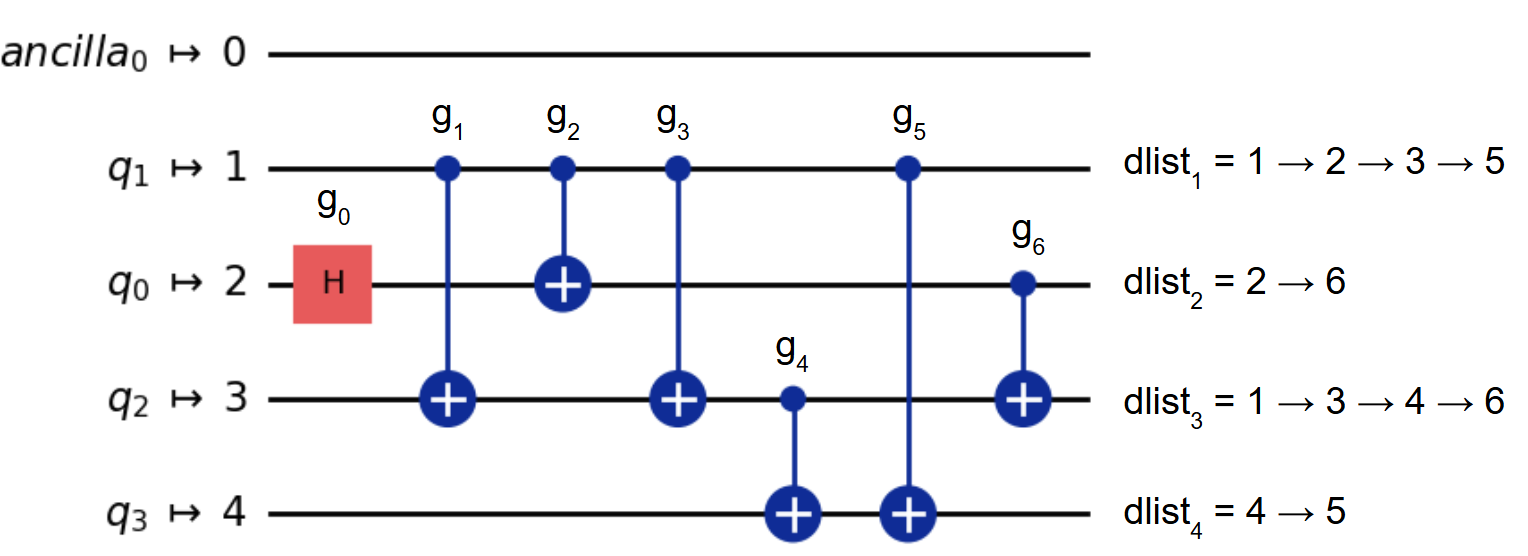
\includegraphics[width=0.7\linewidth]{image/dependency_list.png}
    \caption{The dependency list of a quantum circuit, where dlist\textsubscript{1} contains $g_1, g_2, g_3, \text{and } g_5$, which are two-qubit gates that lie on $q_1$.}
    \label{fig:dependency-list}
\end{figure}

\begin{definition} % done chat
    The effect of a swap gate on a specific two-qubit gate is defined as the change in the nearest neighbour distance of that gate before and after the swap is applied.
\end{definition}
When a swap gate is applied, it alters the nearest neighbour distance for subsequent two-qubit gates that share a logical qubit with the swap. Each swap impacts only one distance, leading to one of three outcomes: the distance can decrease by 1 (positive effect), increase by 1 (negative effect), or remain unchanged (no effect) \cite{zhu_dynamic_2020}. In figure \ref{fig:lookahead-window}, each rectangle represents a two-qubit gate, with $``+"$ indicates a non-negative effect (0 or +1), while $``-"$ signifies a negative effect (-1).

\begin{figure}[h]
    \centering
    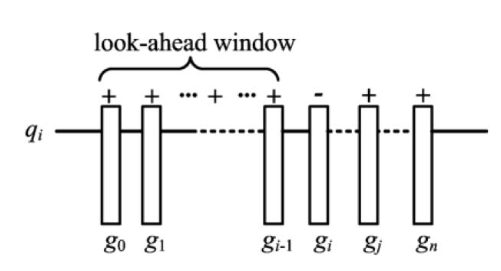
\includegraphics[width=0.5\linewidth]{image/lookahead_window.png}
    \caption{Diagram for the dynamic look-ahead technique. Adapted from \cite{zhu_dynamic_2020}}
    \label{fig:lookahead-window}
\end{figure}

The effect of a swap gate applied to $(Q_i, Q_j)$ changes the nearest neighbour distance of $g_i$, as determined by the logical to physical mapping before the swap $(\pi_1)$ and after the swap $(\pi_2)$.
\begin{equation}
    \text{effect}(\text{SWAP}, g_i) = \text{dist}(g_i, \pi_1) - \text{dist}(g_i, \pi_2)
\end{equation}

\begin{definition}
    The look-ahead technique is a heuristic cost function used to evaluate how effectively a swap gate ensures that the circuit meets connectivity constraints.
\end{definition}
The method used in Qiskit relies on a fixed window size that is determined before the mapping process begins \cite{ibmquantum_lookaheadswap}. This fixed window approach has limitations because it considers a predetermined number of gates across all qubits, regardless of their relevance. Additionally, with a fixed-size window, the heuristic cost function might select a swap gate that helps some gates scheduled later but negatively impacts those that are executed earlier. In extreme cases, the chosen swap could be harmful to current active gates but may be beneficial for future ones, potentially slowing down or even blocking the heuristic algorithm to progress. \\
To overcome these issues, a dynamic look-ahead technique is introduced as the heuristic cost function. This approach evaluates the effect of a swap gate by focusing only on the two-qubit gates directly affected by the swap. It selectively looks ahead at the two logical qubits ($q_i$ and $q_j$) that experience a positive effect, stopping when a negative effect is encountered. As illustrated in Figure \ref{fig:lookahead-window}, lookahead window only considers from $g_0$ to $g_{i-1}$, where the values are non-negative. The look-ahead window sums all the non-negative (1 or 0) effects on the logical qubit $q_L$:
\begin{equation}
    \text{Lookahead}(\text{SWAP}, q_i) = \sum_{g \in \text{window}} \text{effect}(g)
\end{equation}
The value of Lookahead(SWAP) includes both logical qubits $q_i$ and $q_j$ where the swap gate is inserted,
\begin{equation}
    \text{Lookahead}(\text{SWAP}) = \text{Lookahead}(\text{SWAP}, q_i) + \text{Lookahead}(\text{SWAP}, q_j)
\end{equation}
All these definitions are incorporated to Algorithm \ref{alg:lookahead-swap-routing} \mycode{Lookahead Swap Routing}.
\begin{algorithm}[htbp]
\caption{Lookahead Swap Routing}\label{alg:lookahead-swap-routing}
\hspace*{\algorithmicindent} \textbf{Input} Coupling Graph G(V, E), Circuit DAG \\
\hspace*{\algorithmicindent} \textbf{Output} Circuit DAG
\begin{algorithmic}[1]

\Procedure{check gate connectivity}{$g_i$}
    \State $Q_i \gets \pi(q_i)$
    \State $Q_j \gets \pi(q_j)$
    \State $D[Q_i][Q_j]$
    \If{$D[Q_i][Q_j] == 1$}
        \State dlist[$q_i$] pop front
        \State dlist[$q_j$] pop front
        \State new\_dag apply operation back($g_i$)
    \Else
        \State act\_list.append($g_i$)
    \EndIf
\EndProcedure

\item[]

\State dlist[\ ] $\gets$ $g_i$ on $q_n$ iff two-qubit gates
\State new\_dag $=$ dag.copy\_empty()
\State act\_list $= [\ ]$
\For{dag layers} \Comment{traverse circuit depth per level}
    \For{$g_i$ in dag operation nodes}
        \If{$g_i$ is a two-qubit gate of ($q_i, q_j$)}
            \State check gate connectivity($g_i$)
        \Else
            \If{$g_i$ is 'measure' operation}
                \State $C_i \gets q_i$ the corresponding updated $Q_P$ for register
            \EndIf
            \State new\_dag apply operation back($g_i$)    
        \EndIf
    \EndFor
    \While{act\_list is not empty}
        \State check gate connectivity($g_i$)
        \State candidate list $=$ generate possible physical swaps
        \For{swap$(Q_x, Q_y)$  in candidate list}
            \State Lookahead $(\text{swap}(Q_x, Q_y)) = \sum_{g} \text{effect}(Q_x(g)) + \sum_{g} \text{effect}(Q_y(g))$
        \EndFor
        \State highest swap $(Q_x, Q_y)$ $\gets$ max(lookahead)
        \State new\_dag apply operation back(SwapGate$(Q_x, Q_y)$)
    \EndWhile
\EndFor
\end{algorithmic}
\end{algorithm}

\subsection{Lookahead Swap Routing Algorithm}
Figure \ref{fig:swap-trivial-basic} demonstrates the transpilation process using Qiskit \lstinline{TrivialLayout} \cite{ibmquantum_triviallayout} and \lstinline{BasicSwap} \cite{ibmquantum_basicswap} routing methods. The \lstinline{TrivialLayout} assigns virtual qubits to physical qubits by mapping $n$ logical qubits to device qubits $0, 1, ...,, N-1$ in ascending order. The \lstinline{BasicSwap} then performs minimal adjustments by inserting one or more swap gates before a two-qubit gate until the quantum information is located at adjacent physical qubits. \\
In contrast, Figure \ref{fig:swap-lookahead} illustrates the process using the interaction layout from Algorithm \ref{alg:interaction-layout-mapping}. Initially, the algorithm converts the circuit to \acrshort{dag} and creates a dependency list for all two-qubit gates, as shown in Figure \ref{fig:dependency-list}. It then iterates over the \acrshort{dag}'s level layers, checking the gate operation's coupling map distance $D[q_i][q_j]$. If the distance is 1, indicating that the logical qubits are adjacent, the gate is directly applied, and the gate nodes are added to the \acrshort{dag} circuit. However, if the distance is greater than 1, the node is inserted into the active list. \\
The first four layers have a distance of 1, allowing gates $g_0$ through $g_4$ to be executed directly. The next layer includes $g_5 (q_1, q_3)$ and $g_6 (q_0, q_2)$, for which the algorithm generates a list of physical swap candidates for each gate. For gate $g_5$, the swap candidates are $[(Q_2, Q_1), (Q_3, Q_1), (Q_3, Q_4)]$, while gate $g_6$ adds the swap candidate $(Q_1, Q_0)$. The algorithm then calculates the lookahead heuristic value for subsequent gates on the dependency list. If a negative effect is encountered during the iteration, the process terminates, and the lookahead window only considers non-negative values. After the calculation, the swap between $Q_3$ and $Q_1$ has the highest lookahead value. The next step is to recalculate the distance between the new swap positions for the gates. If the gates can now be executed directly, the gate operation is added to the DAG. The final step is to determine the order of the measurement operations to the classical registers, taking into account the updated logical-to-physical qubit mapping after the swaps.

\begin{figure}[htb]
    \begin{subfigure}{0.25\linewidth}
        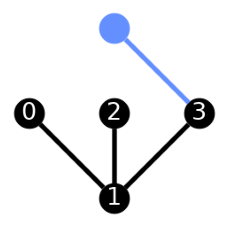
\includegraphics[width=\linewidth]{image/coupling_map_trivial_basic.png}
        \caption{One-to-one mapping}
        \label{fig:one-to-one-mapping}
    \end{subfigure}
    \hfill
    \begin{subfigure}{0.7\linewidth}
        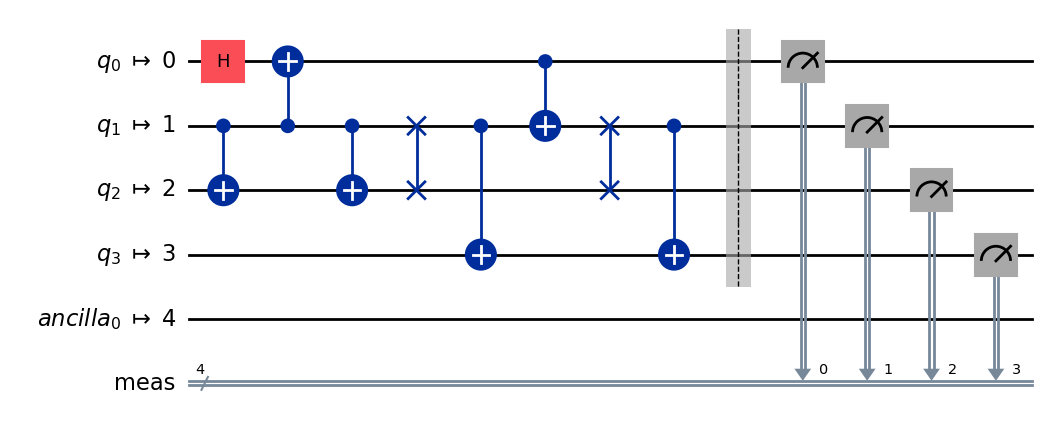
\includegraphics[width=\linewidth]{image/swap_trivial_basic.png}
        \caption{Transpiled quantum circuit with basic swap routing}
        \label{fig:swap-trivial-basic}
    \end{subfigure}
    \hfill
    \begin{subfigure}{0.25\linewidth}
        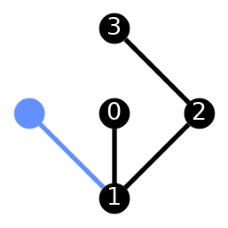
\includegraphics[width=\linewidth]{image/coupling_map_lookahead.png}
        \caption{Interaction layout mapping}
        \label{fig:interaction-mapping}
    \end{subfigure}
    \hfill
    \begin{subfigure}{0.7\linewidth}
        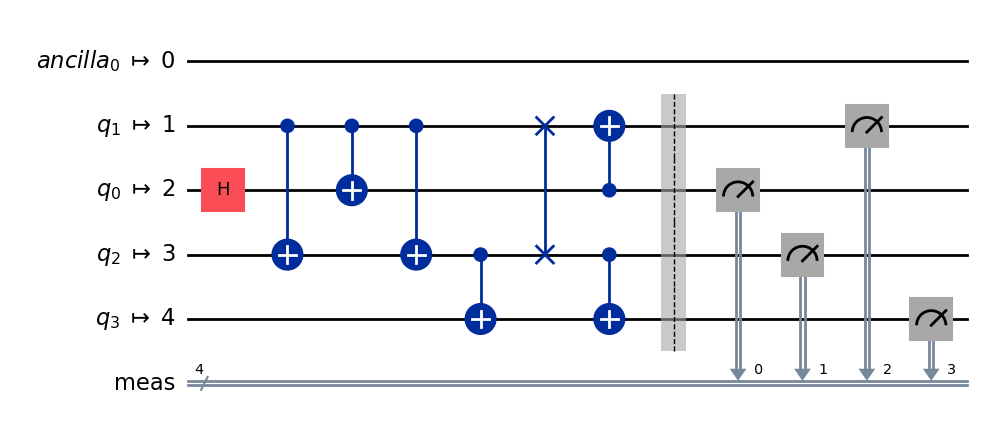
\includegraphics[width=\linewidth]{image/swap_lookahead.png}
        \caption{Transpiled quantum circuit with lookahead swap routing}
        \label{fig:swap-lookahead}
    \end{subfigure}
    \caption{Comparison between layout and routing implementation}
\end{figure}

\subsection{Transformation Pass} % done turnitin
The Pass Manager responsible for routing requires the use of a \lstinline{TransformationPass} \cite{ibmquantum_transformationpass} to modify the \acrshort{dag} structure representing the quantum circuit. This pass manager takes the device's coupling map and the circuit's \acrshort{dag} as inputs and modifies the \acrshort{dag} by inserting the necessary swap gates to ensure that the circuit adheres to the hardware coupling constraints. The output of this process is a transpiled quantum circuit that is compatible with the physical device and ready for execution.

\section{Integration}
\subsection{Staged Pass Manager} % done chat, turnitin
The final step involves integrating both Algorithm \ref{alg:interaction-layout-mapping} \mycode{Interaction Layout Mapping} and Algorithm \ref{alg:lookahead-swap-routing} \mycode{Dynamic Lookahead Swap Routing} into the Staged Pass Manager. In this pass manager, the \lstinline{init} stage unrolls gates involving more than three qubits, and \lstinline{layout} applies the most effective interaction layout mapping. The \lstinline{routing} generates the minimal number of SWAP gates required to satisfy the device's coupling constraints. The final stage, \lstinline{translation}, converts the logical gates into the available basis gate set for the selected device backend. By employing this staged pass manager, the initial quantum circuit is fully translated and optimized for execution on the target backend. \\
For instance, the initial circuit shown in Figure \ref{fig:circuit-init} has a circuit size of 11 and a circuit depth of 6. When using the \lstinline{TrivialLayout} and \lstinline{BasicSwap} methods, as depicted in Figure \ref{fig:swap-trivial-basic}, the circuit size increases to 17 and depth to 13 (Figure \ref{fig:routing-basic-swap}). In contrast, the \lstinline{InteractionLayout} and \lstinline{LookaheadSwap} methods, as shown in Figure \ref{fig:swap-lookahead}, produce a more compact circuit with a size of 14 and a depth of 9 (Figure \ref{fig:routing-lookahead}).

\begin{figure}[htb]
    \centering
    \begin{subfigure}{0.8\linewidth}
        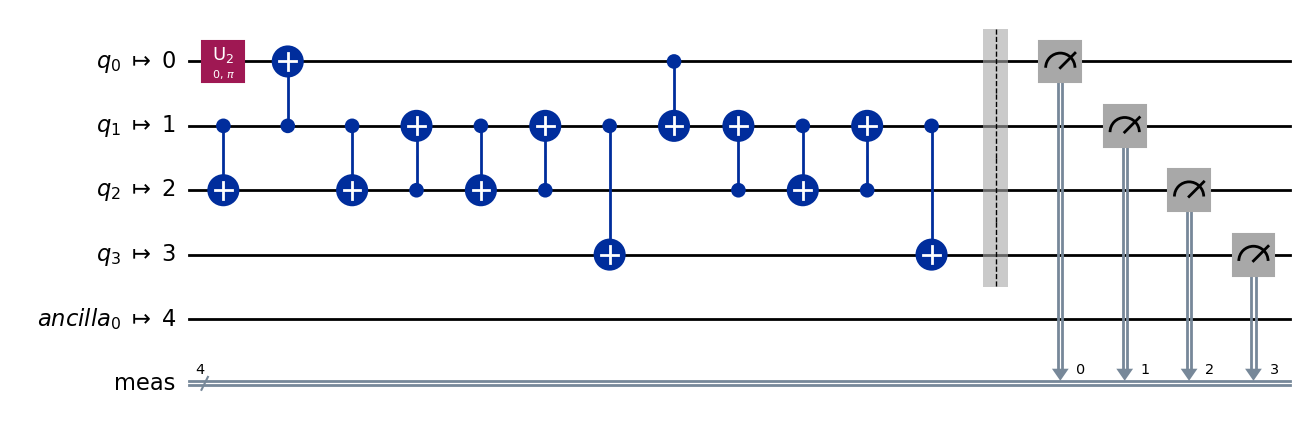
\includegraphics[width=\linewidth]{image/final_trivial_basic.png}
        \caption{Translated final layout with \lstinline{BasicSwap} routing, with additional 2 SWAPs}
        \label{fig:routing-basic-swap}
    \end{subfigure}
    \begin{subfigure}{0.8\linewidth}
        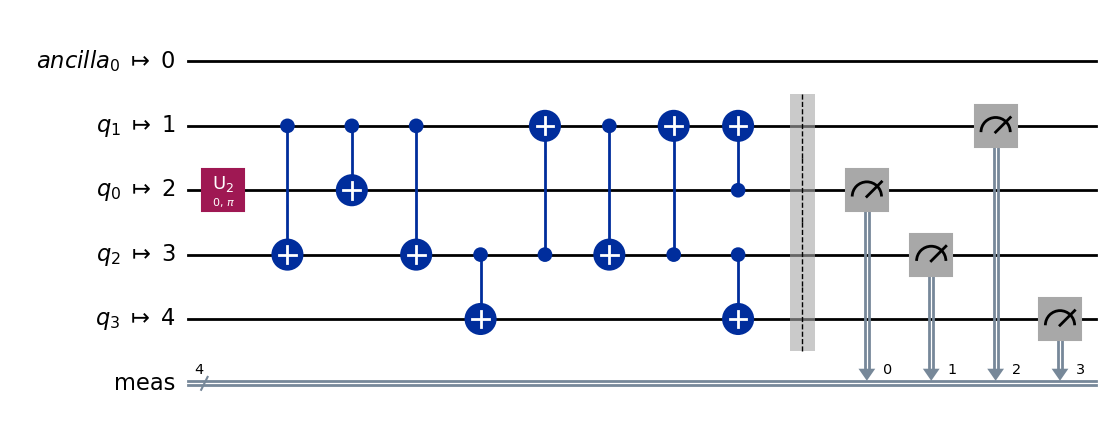
\includegraphics[width=\linewidth]{image/final_lookahead.png}
        \caption{Translated final layout with \lstinline{Lookahead} routing, with additional 1 SWAP}
        \label{fig:routing-lookahead}
    \end{subfigure}
    \caption{Comparison for swap gate routing methods}
\end{figure}

\subsection{Verification} % done chat, turnitin
The verification process involves retrieving the results of a quantum computation after a job has been executed on a quantum device or simulator. For this work, \lstinline{GenericBackend2} \cite{ibmquantum_genericbackendv2} is used, and the backend is run without noise. The result is returned as a dictionary, where the keys represent the bitstrings of the measured qubits, and the values represent the number of times each bitstring was measured. This output allows for the analysis of the probability distribution of the qubit states after the quantum circuit has been executed. \\
The \lstinline{Result} class \cite{ibmquantum_result} of the transpiled quantum circuit, run on Qiskit's preset pass manager, is then compared with the result obtained from the algorithm's swap implementation. It is observed that several of the highest occurrences are identical in both cases (Figure \ref{fig:plot-basic} and Figure \ref{fig:plot-lookahead}), indicating consistency between the two methods, as shown in Appendix \ref{app:verification-probability}.